\documentclass[
  journal=largetwo,
  manuscript=Laboratorio-Numero-02,
  year=2024,
  volume=1
]{cup-journal}

\usepackage{amsmath}
\usepackage[nopatch]{microtype}
\usepackage{booktabs}

\title{Título del laboratorio}

\author{P. Araya}
\affiliation{C1, Universidad Católica del Norte, Coquimbo, Coquimbo, Chile}
\email[P. Araya]{paulo.araya02@alumnos.ucn.cl}

\author{G. Guzman}
\affiliation{C1, Universidad Católica del Norte, Coquimbo, Coquimbo, Chile}
% si son del mismo paralelo solo aparecerá una vez.
% \alsoaffiliation{Joint first authors}


\addbibresource{example.bib}

\keywords{keyword entry 1, keyword entry 2, keyword entry 3} %% en minúsculas

\begin{document}

\begin{abstract}
El resumen es una de las partes más importantes del artículo científico porque comunica en forma rápida y precisa el contenido básico del artículo sin tener que recurrir al resto de la información. El resumen es una síntesis de un solo párrafo (No excede de 100 ó 150 palabras) del objetivo de la práctica y su conclusión de su resultado principal. El resumen de un artículo científico no es el recuento de antecedentes, tampoco es una revisión histórica, ni el análisis o comentario sobre el artículo. No se elabora antes de terminar el artículo.\\

\textbf{Lo mismo pero en inglés.}
\end{abstract}

\section{Introducción}

La introducción debe responder a la pregunta de ¿porqué se ha hecho este trabajo?, es una descripción ampliada del propósito u objetivo del trabajo, así como aspectos generales relevantes (breve descripción histórica). También deben consignarse aquí las hipótesis que se ponen a prueba en el experimento así como también los objetivos del trabajo desarrollado.

\section{Marco teórico}

Breve fundamentación teórica del experimento~\autocite{key-Arthur} Explicación de las ecuaciones que se usan en el experimento.  Cuando estemos revisando modelos de machine learning se consideraría como explicar el clasificador que se va a utilizar: Hipótesis (lineal o no lineal), función de pérdida e hiperparámetros. No más de una columna de página. Debe contener referencias.

\section{Materiales y métodos}
En esta sección se responde a la pregunta de ¿cómo se ha hecho el estudio?. Descripción de las técnicas experimentales usadas, apoyadas en dibujos, gráficas o ejemplos que ayuden a visualizar el experimento. En concreto, tienen que describir o explicar los datos que utilizaron y cómo evaluarán si los resultados son o no positivos. Máximo una plana de extensión.

\begin{table}[]
    \centering
\begin{tabular}{|llll|}
\hline
\multicolumn{4}{|c|}{Stage: Corridor} \\ \hline
\multicolumn{4}{|l|}{Hyperparameters:} \\ \hline
\multicolumn{1}{|c|}{\textbf{Metric}} & \multicolumn{1}{c|}{\textbf{k}} & \multicolumn{1}{c|}{\textbf{MAE}} & \multicolumn{1}{c|}{\textbf{MSE}} \\ \hline
\multicolumn{1}{|l|}{Min MSE} & \multicolumn{1}{l|}{6} & \multicolumn{1}{l|}{\textbf{$0.1049\pm 0.0217$}} & $0.1049\pm 0.0217$ \\ \hline
\multicolumn{1}{|l|}{Min MAE} & \multicolumn{1}{l|}{} & \multicolumn{1}{l|}{} &  \\ \hline
\end{tabular}
\caption{Tabla de Ejemplo}
    \label{tab:my_label}
\end{table}

\begin{figure}[!ht]
    \centering
    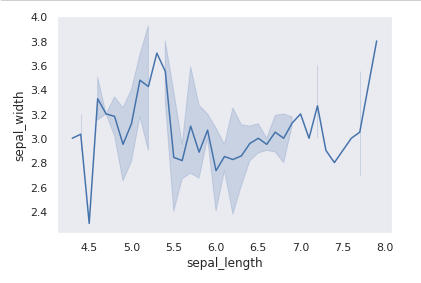
\includegraphics[width=0.8\textwidth]{fig/graphs/seaborntutorialstylingplots.png}
    \caption{Caption}
    \label{fig:my_label}
\end{figure}

\section{Resultados y discusión}

Esta sección es el corazón del manuscrito, donde la mayoría de los lectores irán después de leer el resumen. Aquí deben consignarse la tabla de datos de las mediciones directas realizadas en el laboratorio. Las tablas de datos, ilustraciones y gráficas, se identifican con números de series y una descripción concisa y clara. Los encabezados de las columnas deben contener el nombre de la variable, su símbolo y unidades de medida. Junto a cada entrada numérica debe figurar la respectiva incertidumbre, a menos que un análisis de incertidumbre separado que clasifique la precisión de las mediciones. Las gráficas deben tener los ejes coordenados debidamente identificados con sus unidades. Se debe efectuar un análisis riguroso de los datos, las consecuencias, de las observaciones y de las implicaciones físicas de las relaciones entre variables. Si hay un análisis por separado de las incertidumbres experimentales, por métodos estadísticos[2] o no estadísticos, debe incluirse en esta sección. Máximo una plana de extensión.

\section{Conclusiones}

La justificación para escribir un informe de laboratorio la constituyen las conclusiones que obtenemos a partir de nuestras observaciones y medidas. Se discute el acuerdo o la discrepancia entre el modelo propuesto y el comportamiento observado, así como la validez de las hipótesis planteadas. Finalmente, se procede a efectuar interpretaciones o conjeturas sobre las razones de las discrepancias y a sugerir refinamientos, bien sea del modelo o del procedimiento experimental, que permitan dilucidar los interrogantes a los que el experimento dio lugar. Información extraída de los resultados obtenidos. Por ejemplo, este problema funciona mejor
con un clasificador lineal, con kernel de tipo A y datos normalizados con la técnica X.
También, se puede observar que el ruido afecta el rendimiento del clasificador y que en
ciertas ocasiones conviene…
No más de una columna de página.

%\endnote in some journals will behave like \footnote; and \printendnotes will not output anything.
\printendnotes
%se le recomienda para la bibliografía usear como guía la forma de este lab utilizando el archivo example.bib como referencia. Si desea no usarlo, sus referencias deben ser en APA.
\printbibliography

\appendix

\section{Anexos}
Aquí consigne las relaciones de incertidumbres usadas, si son muchas tablas y gráficos y los considera importante los puede consignar aquí.

\end{document}